\documentclass{article}
\usepackage{graphicx}
\usepackage{wrapfig}
\usepackage{subcaption}
\usepackage[margin=1in]{geometry}
\usepackage{amsmath} % or simply amstext
\usepackage{siunitx}
\usepackage{booktabs}
\usepackage[export]{adjustbox}
\newcommand{\angstrom}{\textup{\AA}}
\usepackage{cleveref}
\usepackage{booktabs}
\usepackage{gensymb}
\usepackage{float}

\begin{document}
  \graphicspath{{./figures/}}
  
  % Context: At this point in the manuscript, I have already narrowed the
  % systems down to a disordered structure and the ordered sandwiched configuration
  % I've named them Basin A and Basin B for simplicity. A - ordered, B - disordered
  % I don't call them the ordered and disordered basins because I think that can 
  % be misleading 
  % I'm open to other naming ideas. 
  We can not immediately classify Basin A and Basin B as separate phases.
  \begin{itemize}
	\item To prove the existence of two phases we need evidence of a
	a first order phase transition.
	\item A first order phase transition can be denoted by a discontinuity
        of some order parameter in response to an external condition such as
	temperature.
	\item We chose three easily measurable order parameters: the distance
	between pores, the membrane thickness and the ratio of pore radius to
	the uncertainty in pore radius.  % BJC: these may change
        \item The pore radius is divided by its uncertainty as a way of quantifying
        the degree to which monomers obstruct the pore region.
  \end{itemize}

  Basin B is the dominant configuration at higher temperatures.
  \begin{itemize}
	\item We linearly ramped the temperature of a system in Basin A 
	from 280K to 340K over 100 ns.
        \item Visually, there is a distinct change in pore structure from one
        characteristic of Basin A (Figure~\ref{fig:280K_pore}) to one characteristic of
        Basin B (Figure~\ref{fig:340K_pore}).
        \item The slope of all order parameters changes between 315K and 325K
	(\Cref{fig:p2p_tramp,fig:thickness_tramp,fig:order_tramp}) indicating the
        possibility of an abrupt change in system ordering.
        \item Our 100 ns temperature ramp was likely too fast and caused the system
        to suffer from hysteresis.
  \end{itemize}

  In an attempt to mitigate hysteresis, we performed a slow, stepwise temperature ramp.
  \begin{itemize}
        \item Starting from a sandwiched structure equilibrated at 280K, the system
        temperature was raised to 300K and allowed to equilibrate for 200 ns.
        \item At the end of 200 ns, the temperature was raised 5K and equilibrated
        again for 200 ns.
        \item We continued raising the temperature by 5K and equilibrating for 200 ns
        until the system was equilibrated for 200 ns at 320K.
	\item The same process was repeated with a system equilibrated in Basin B and used
	as a benchmark for comparison. 
  \end{itemize}

  \begin{figure}
        \centering
        \begin{subfigure}[b]{0.475\textwidth}
                \centering
                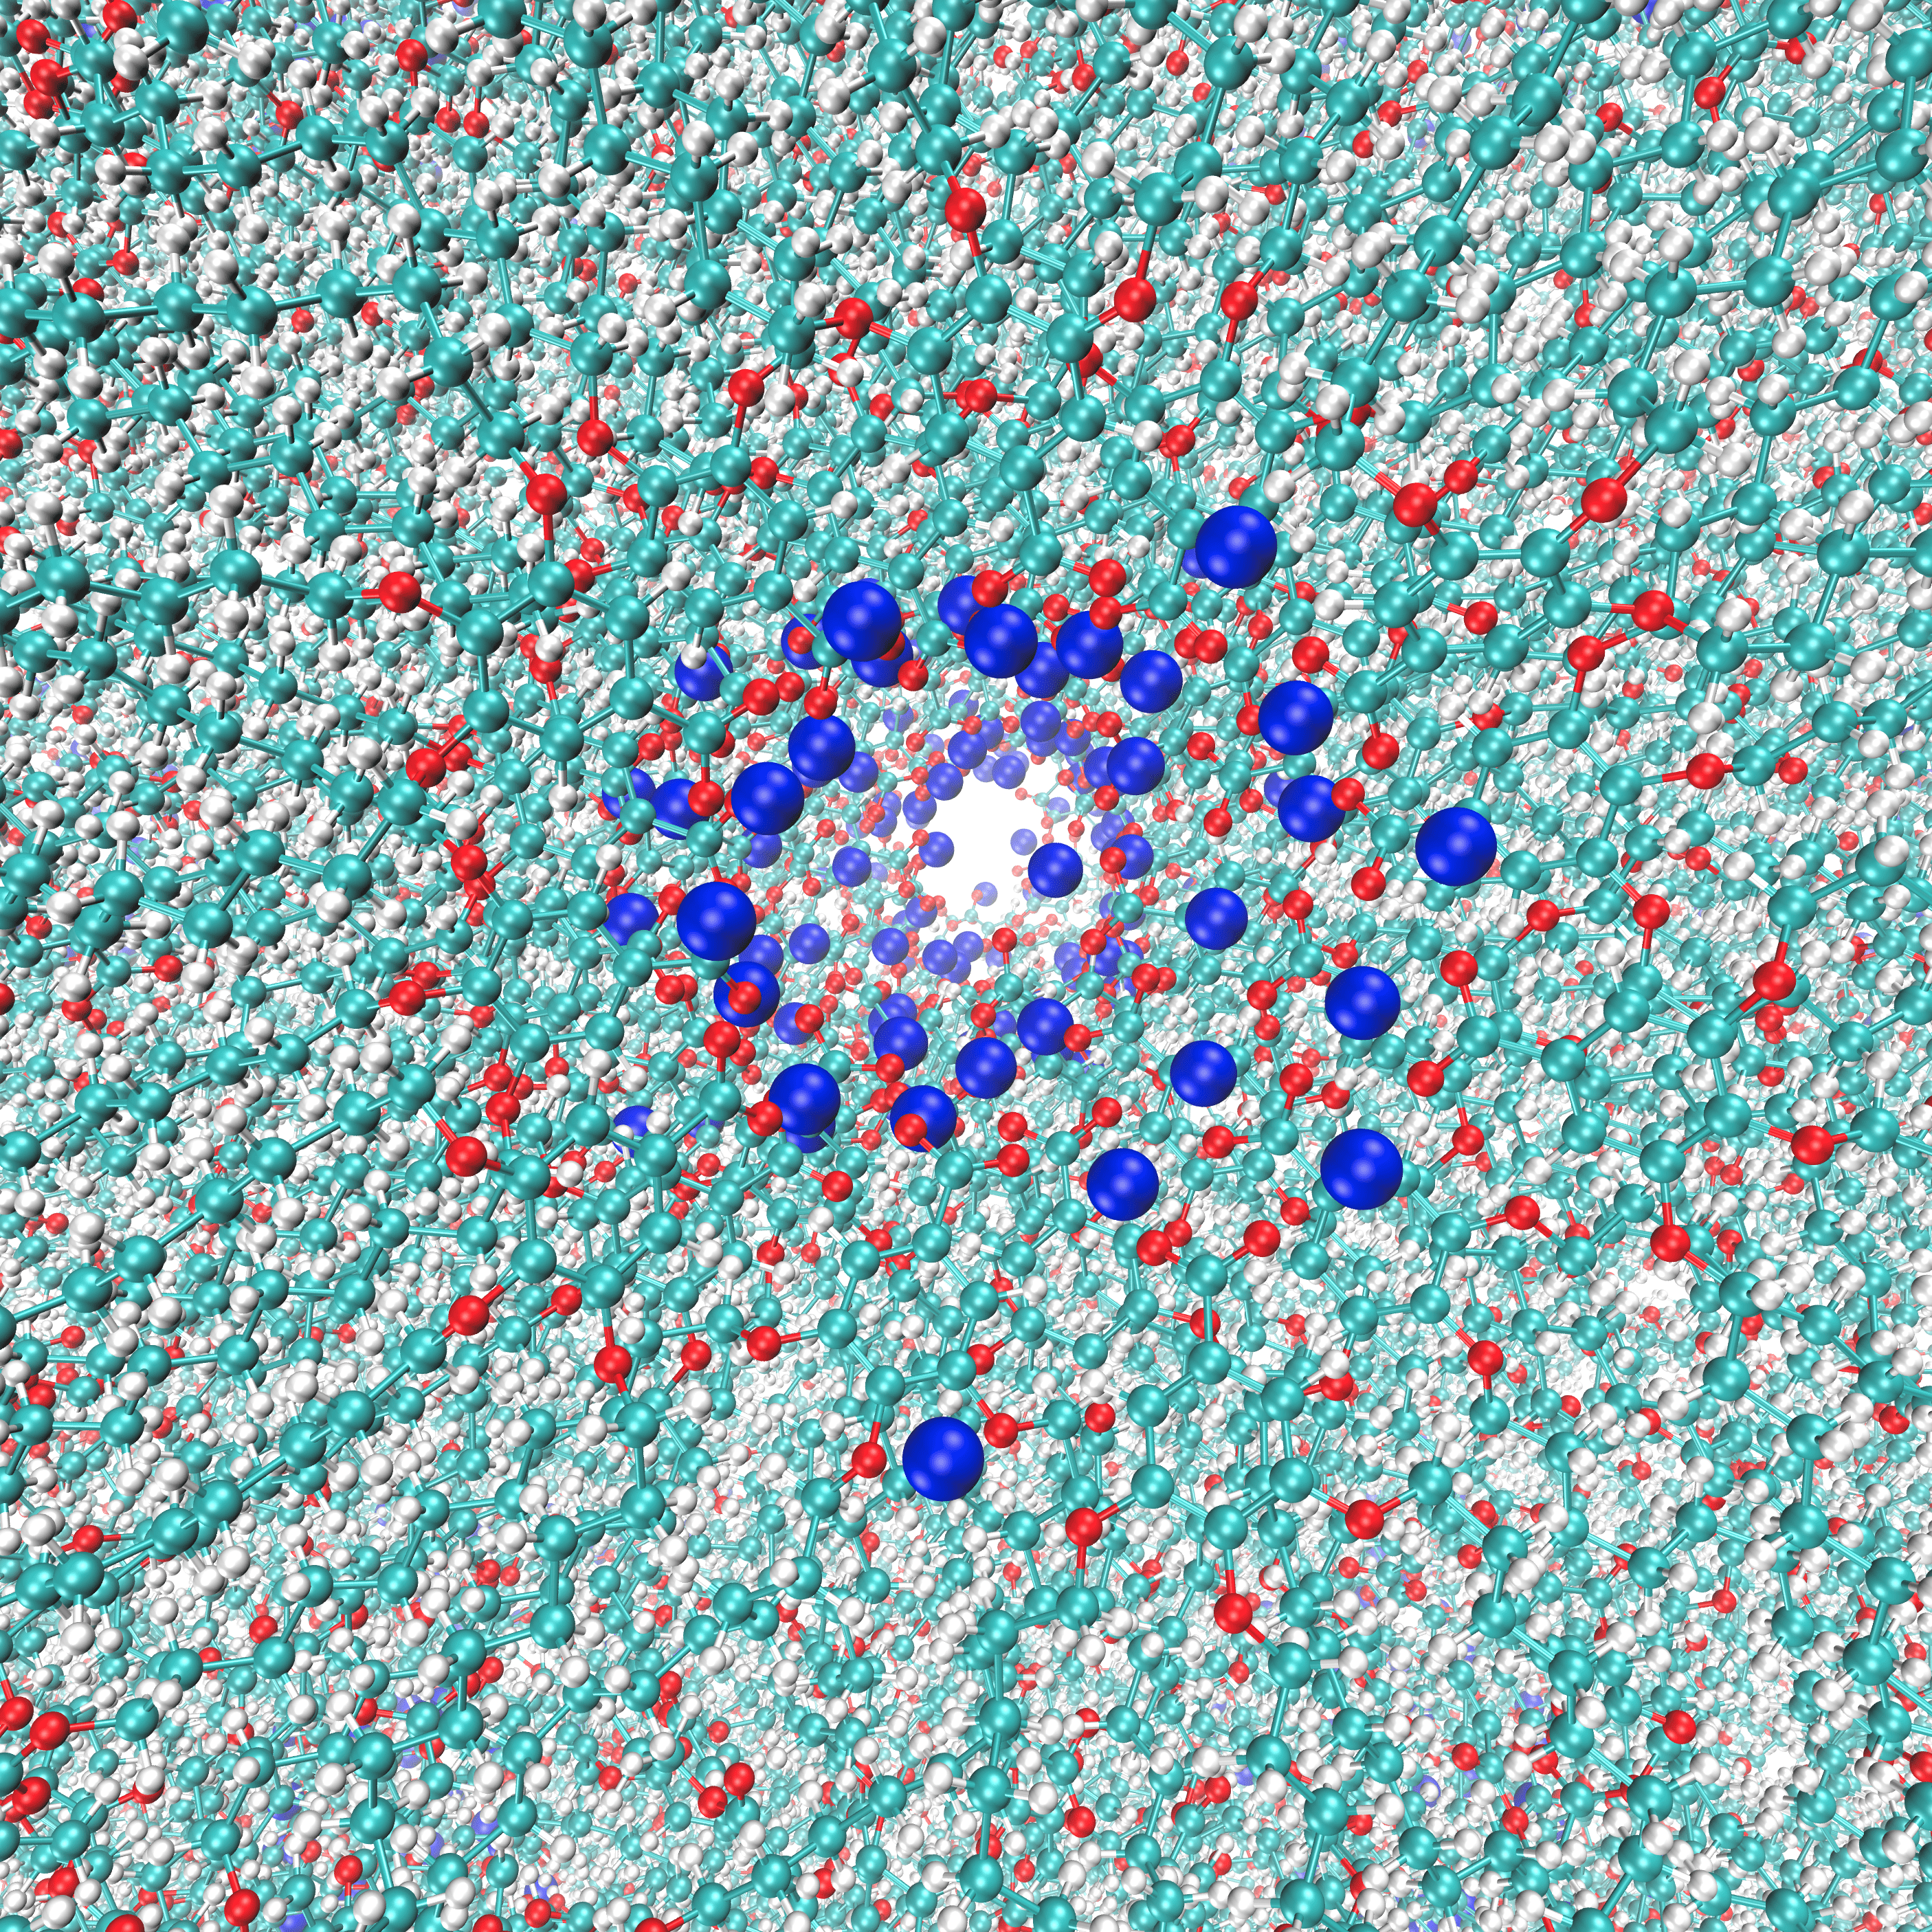
\includegraphics[width=\textwidth]{280K_tramp_close.png}
                \caption{}\label{fig:280K_pore}
        \end{subfigure}
        \begin{subfigure}[b]{0.475\textwidth}
                \centering
                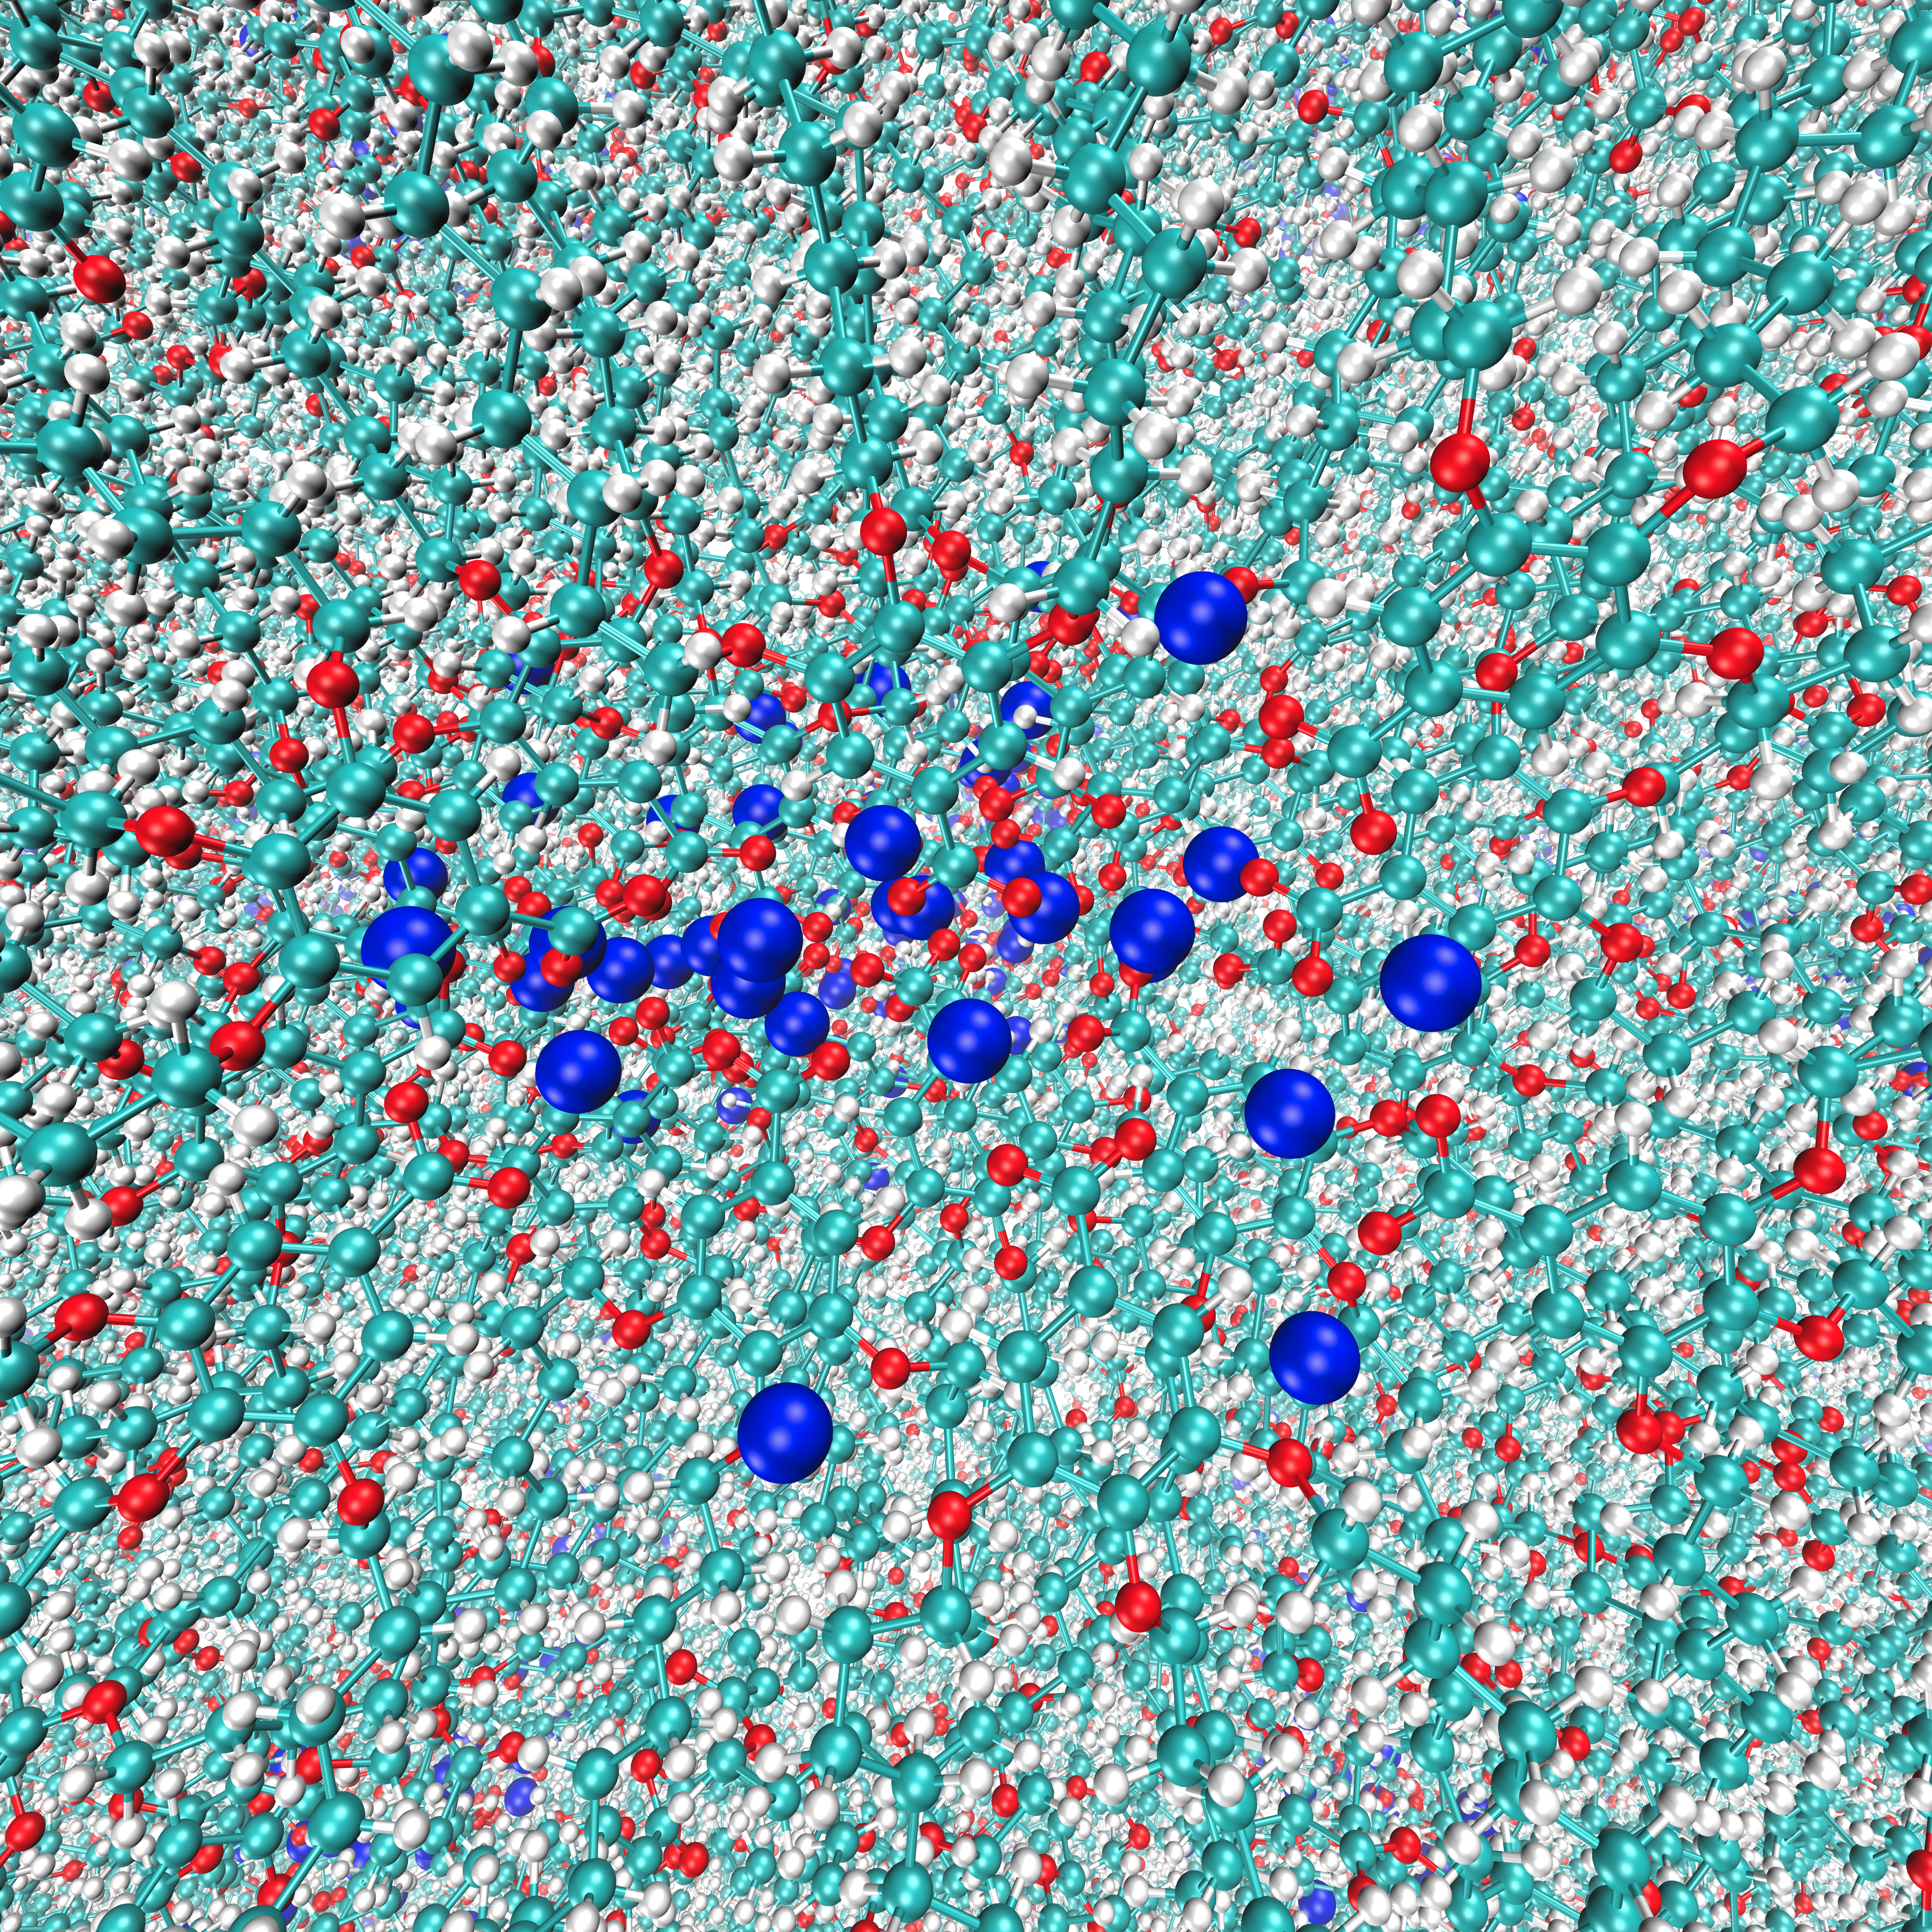
\includegraphics[width=\textwidth]{340K_tramp_close.png}
                \caption{}\label{fig:340K_pore}
        \end{subfigure}
        \vskip\baselineskip
        \begin{subfigure}[b]{0.325\textwidth}
                \centering
                \includegraphics[width=\textwidth]{p2p_tramp.png}
                \caption{}\label{fig:p2p_tramp}
        \end{subfigure}
        \begin{subfigure}[b]{0.325\textwidth}
                \centering
                \includegraphics[width=\textwidth]{thickness_tramp.png}

                \caption{}\label{fig:thickness_tramp}
        \end{subfigure}
        \begin{subfigure}[b]{0.325\textwidth}
                \centering
                \includegraphics[width=\textwidth]{order_tramp.png}
                \caption{}\label{fig:order_tramp}
        \end{subfigure}
        \caption{(a) The open pore structure exhibited by a structure equilibrated
        at 280K is characteristic of Basin A. (b) The closed pore structure with
        a high degree of radial disorder exhibited when the structure in (a) is
        heated to 340K is characteristic of Basin B. (c) A plot of distance between pores
        vs. temperature changes slope near 325K. (d) A plot of membrane thickness vs.
        temperature changes slope near 325K. (e) The plot of the ratio of pore radius to
        its uncertainty changes slope near 315K.}\label{fig:tramp}
  \end{figure}

  Basin A and Basin B are two configurationally metastable basins.
  \begin{itemize}
        \item There is litle change in disordered phase properties during the 
        temperature ramp.
	\item We observed smooth changes in order parameters as temperature
        of the Basin A system was increased implying that we cannot claim the
	existence of two phases (Figure~\ref{fig:phase_transition}).
	\item Qualitatively, the pore structure of the Basin A system becomes
        comparable to one characteristic of Basin B as temperature is raised. (\Cref{fig:BasinA_280K_pore,fig:BasinA_340K_pore})
	\item The Basin A system does not converge to the same order parameter
	values as Basin B, however it is trending towards Basin B values. (\Cref{fig:p2p_step,fig:thickness_step,fig:order_step})
	\item To resolve the quanitative discrepancy, we would need a slower 
	temperature ramp
	\item Since there are no abrupt changes in any order parameter along the 
	trajectory, we can conclude that the two basins are not separate phases
	\item Basin A is the closest match to what is seen experimentally
	\item Basin B is likely an intermediate between the Col\textsubscript{h} 
	phase and isotropic phase
	\item Basin B is present in our simulations at lower temperatures 
	because our model lacks sufficient pi-pi iteractions necessary to 
	stabilize the system into Basin A. 
  \end{itemize} 

  \begin{figure}
        \centering
	% BJC: I'll get actual pictures of the system here. I'm not sure how 
	% necessary this figure is though. It could go in the supplemental 
	% information and I can reference the pictures in the previous figure
	% since they show basically the same idea : Ordered vs. disordered pore
	% Alternatively, I could show two diffraction patterns here from the 
	% beginning and end temperature 
        \begin{subfigure}[b]{0.475\textwidth}
                \centering
                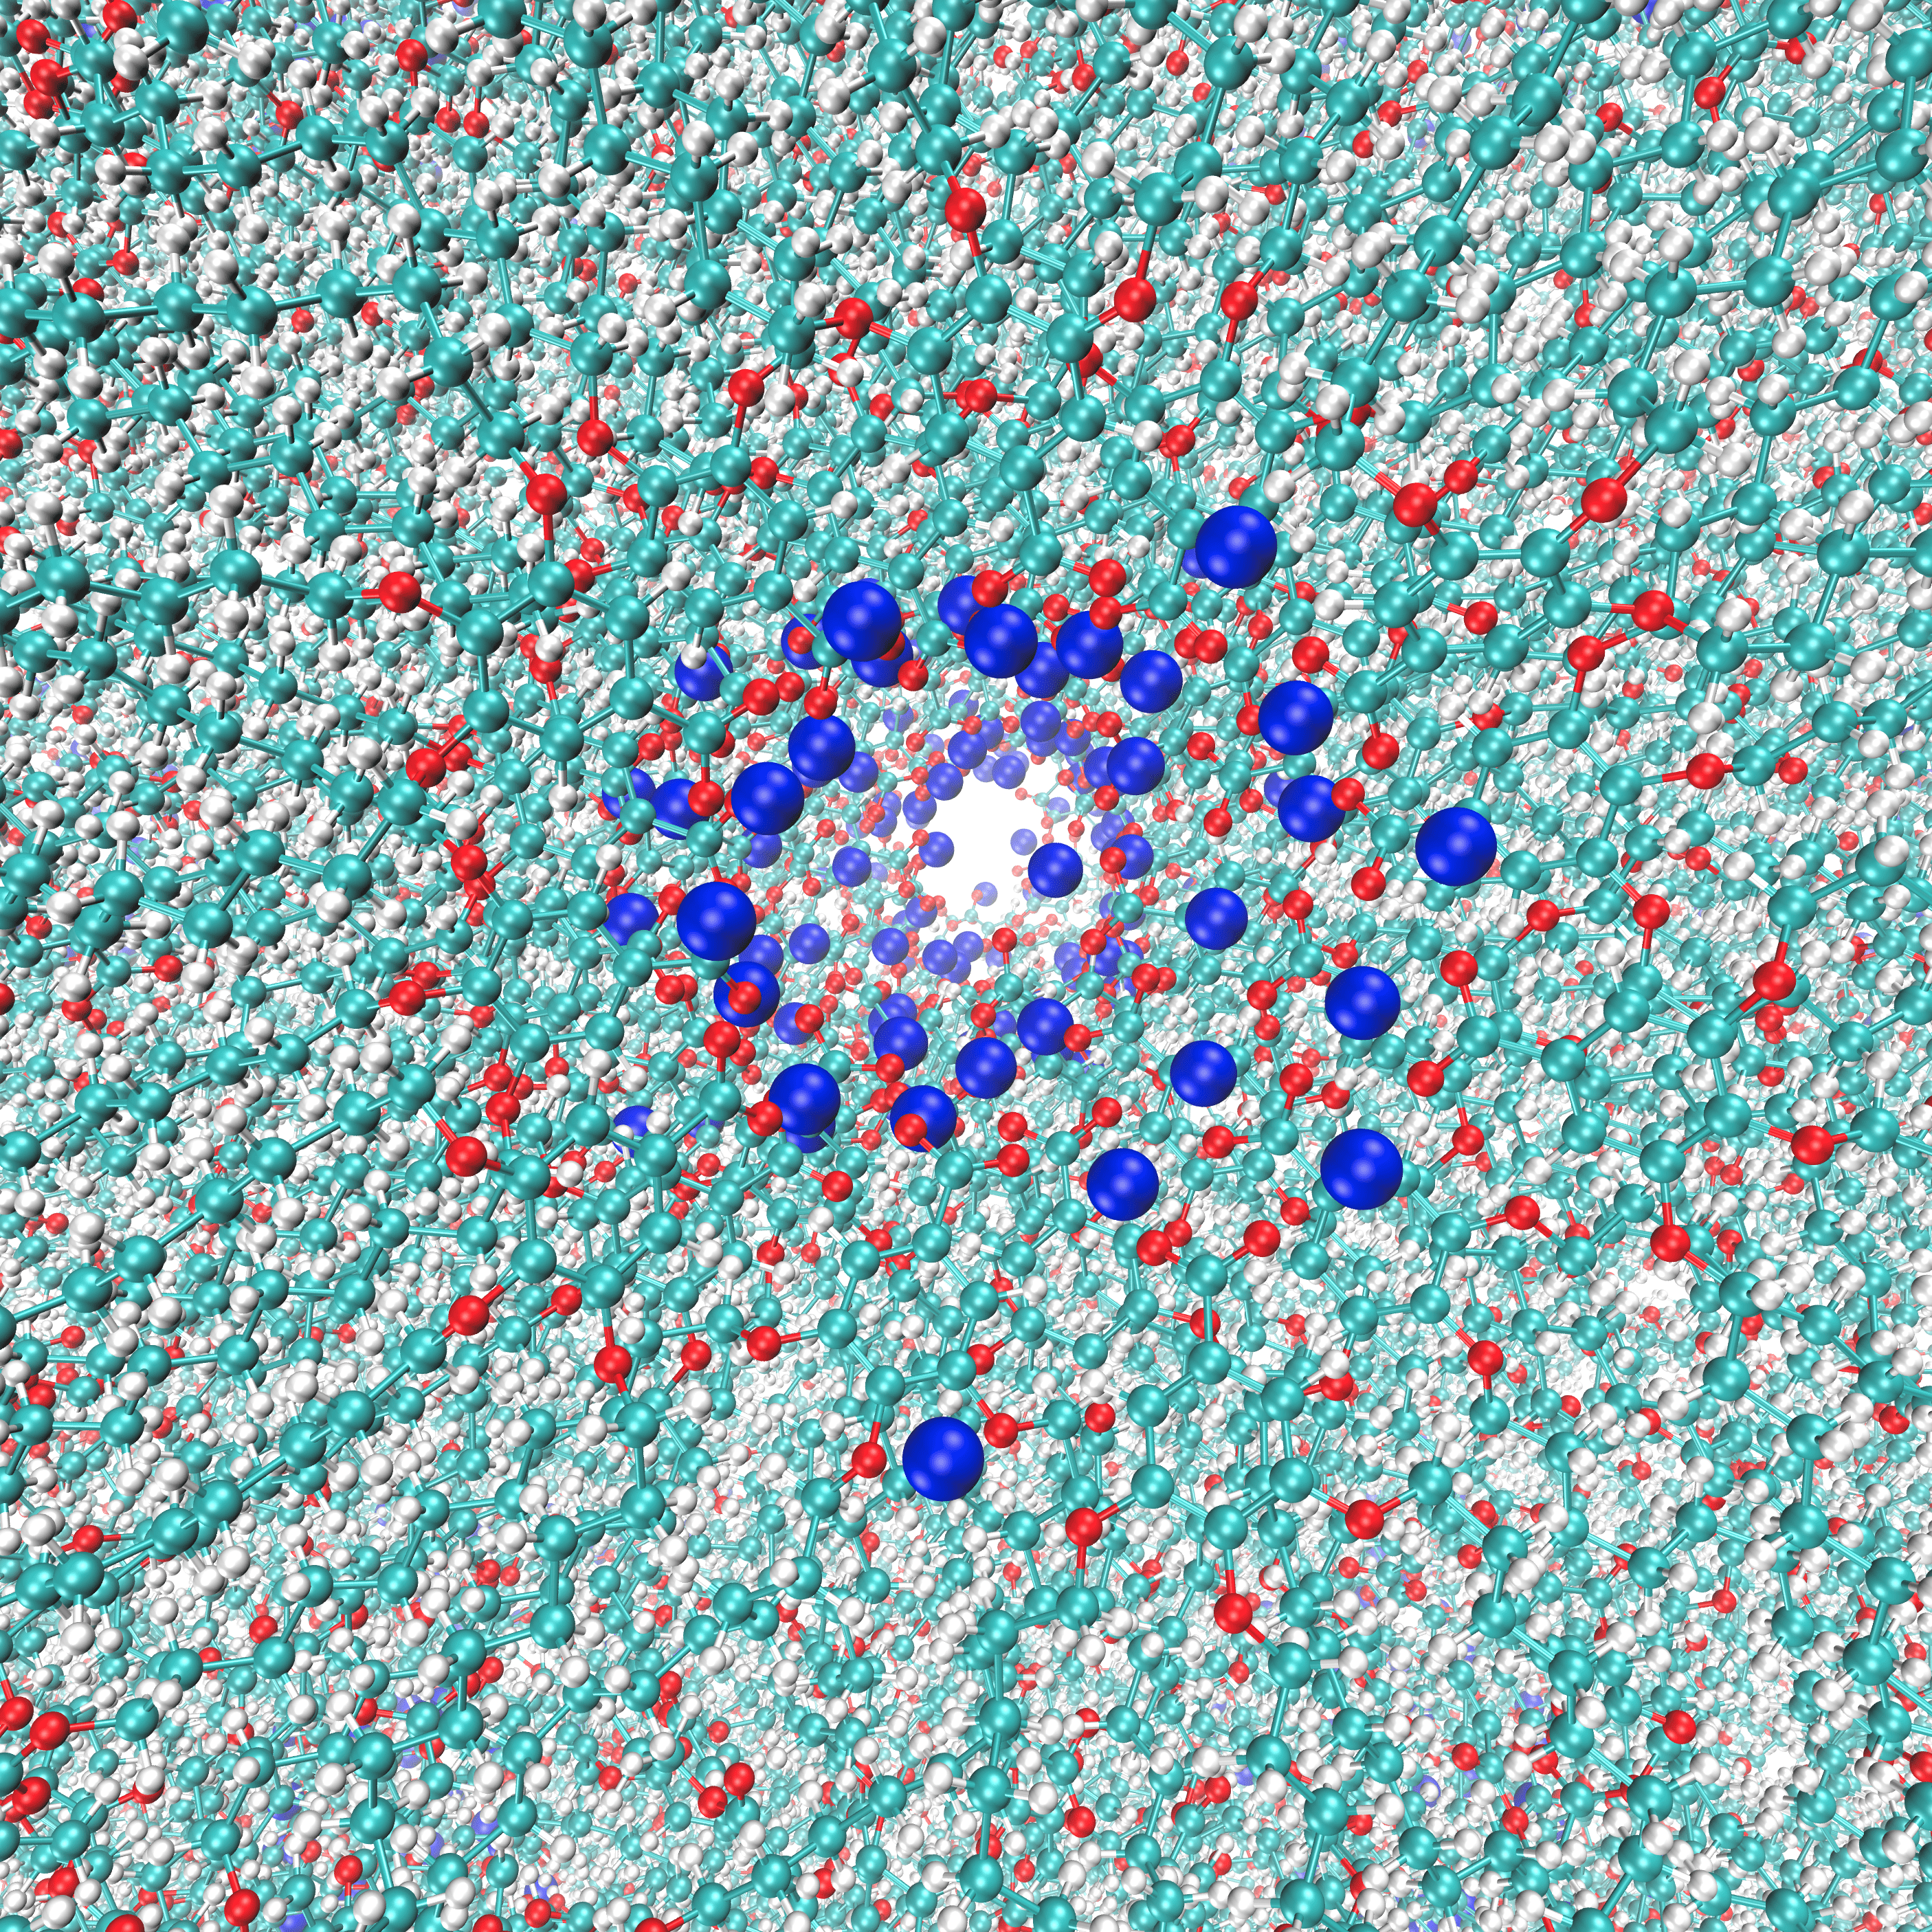
\includegraphics[width=\textwidth]{280K_tramp_close.png}
                \caption{}\label{fig:BasinA_280K_pore}
        \end{subfigure}
        \begin{subfigure}[b]{0.475\textwidth}
                \centering
                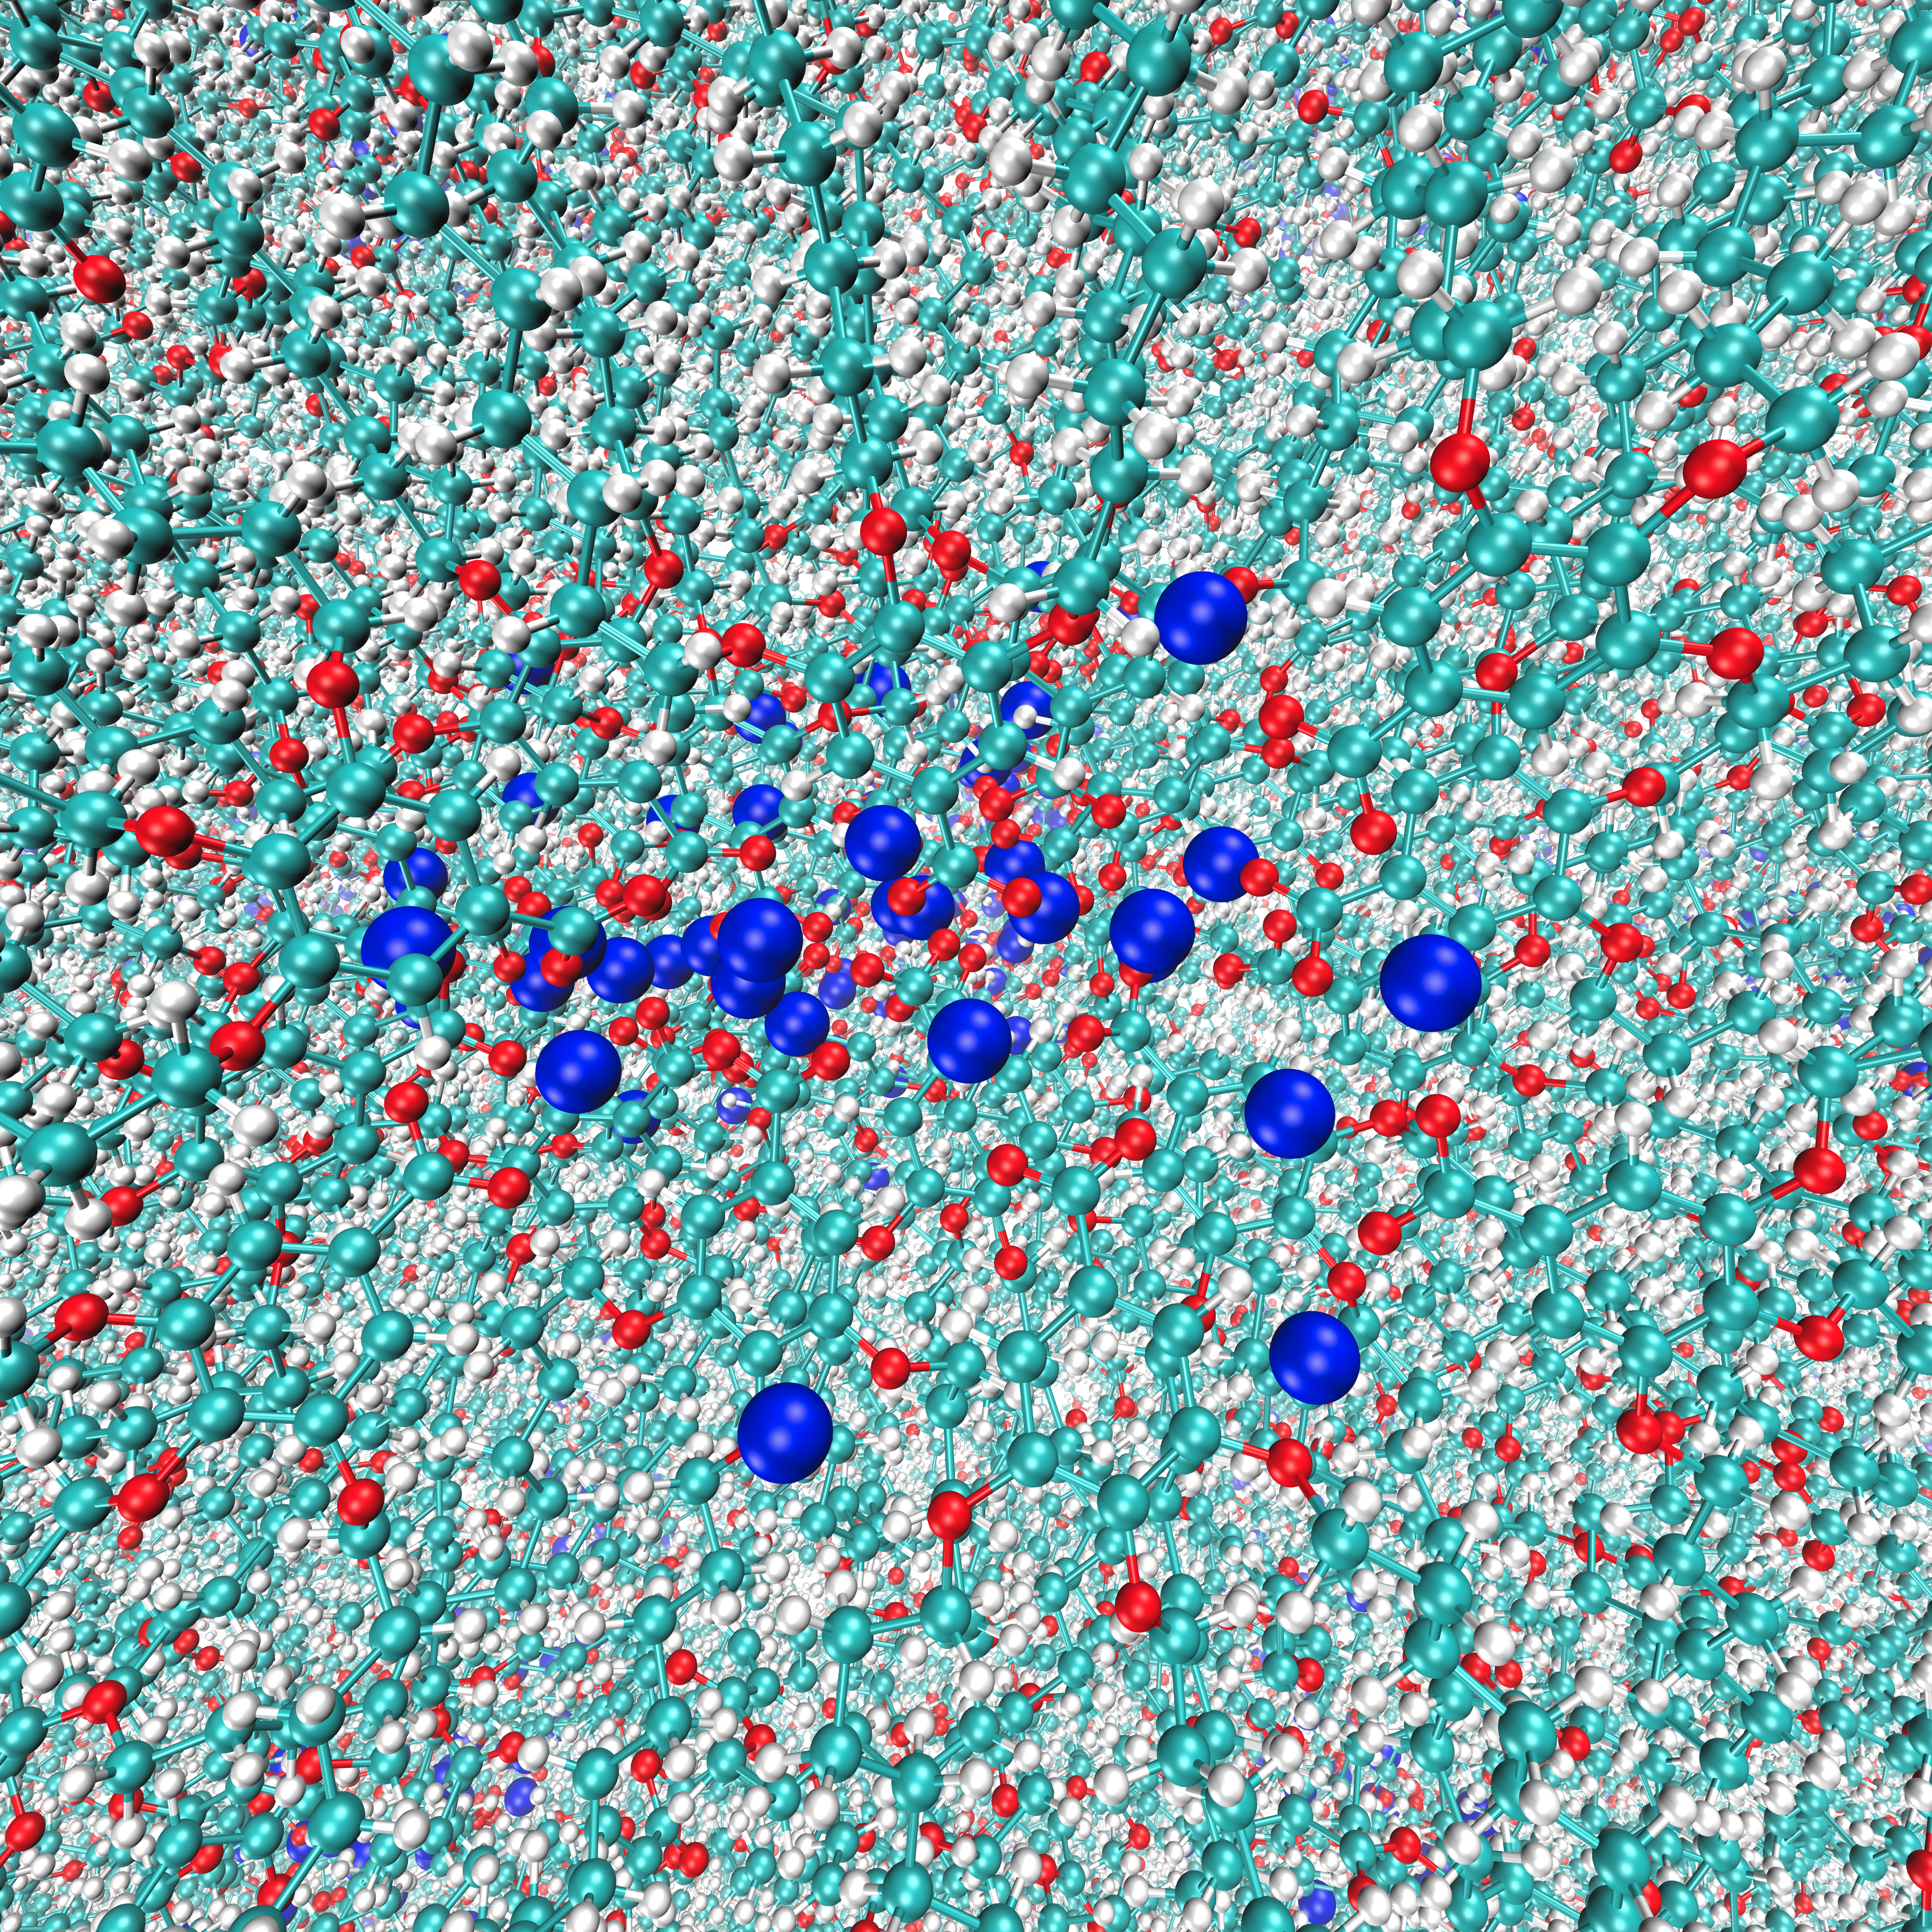
\includegraphics[width=\textwidth]{340K_tramp_close.png}
                \caption{}\label{fig:BasinB_340K_pore}
        \end{subfigure}
	\vskip\baselineskip
        \begin{subfigure}[b]{0.325\textwidth}
                \centering
                \includegraphics[width=\textwidth]{p2p_layered.png}
                \caption{}\label{fig:p2p_step}
        \end{subfigure}
        \begin{subfigure}[b]{0.325\textwidth}
                \centering
                \includegraphics[width=\textwidth]{thickness_layered.png}

                \caption{}\label{fig:thickness_step}
        \end{subfigure}
        \begin{subfigure}[b]{0.325\textwidth}
                \centering
                \includegraphics[width=\textwidth]{order_layered.png}
                \caption{}\label{fig:order_step}
        \end{subfigure}
	\caption{(a) At 280K, the system is in a configuration reminiscent of
	Basin A. (b) At 335K, the system resembles a Basin B configuration. (c) The pore
	spacing of Basin A decreases with temperature approaching the value 
	exhibited by Basin B. (d) The thickness of Basin A increases smoothly with 
	temperature but is far from the Basin B value. Longer equilibrations at 
	each temperature are needed to allow the system to fully expand. (e) The ratio 
	of pore radius to uncertainty for Basin A changes smoothly with temperature,
	converging to a value below that exhibited by Basin B.}\label{fig:phase_transition}
  \end{figure}

\end{document}
